\chapter{Voorgaand werk}
\label{hoofdstuk:voorgaand-werk}
Raytracing vereist acceleratiestructuren om efficiënt driehoeken in de scene te kunnen zoeken.
Dit hoofdstuk start met een algemene uitleg over acceleratiestructuren en wijdt dan uit over één specifieke acceleratiestructuur: de \textit{Binary Space Partitioning} ($\symBSP$) boom.
De varianten van de $\symBSP$ boom worden één voor één besproken.
% TODO

\section{Basisconcept}
    
    % TODO: raytracing
    \paragraph{Ray tracing}
    \textit{Ray tracing} is een computergrafiek techniek voor fysisch gebaseerd renderen. Het vormt een beschrijving van een 3D scene om tot een fotorealistische 2D afbeelding. Een camera wordt op een bepaalde positie in de scene geplaatst en een afbeeldingsvlak, opgedeeld in pixels, wordt ervoor geplaatst. Door elke pixel worden één (of meerdere stralen) gestuurd. Deze stralen worden zichtstralen genoemd en de kleur van hun dichtste intersectiepunt met de scene, bepaalt de kleur van de pixel.\\

    \begin{figure}
        \centering
        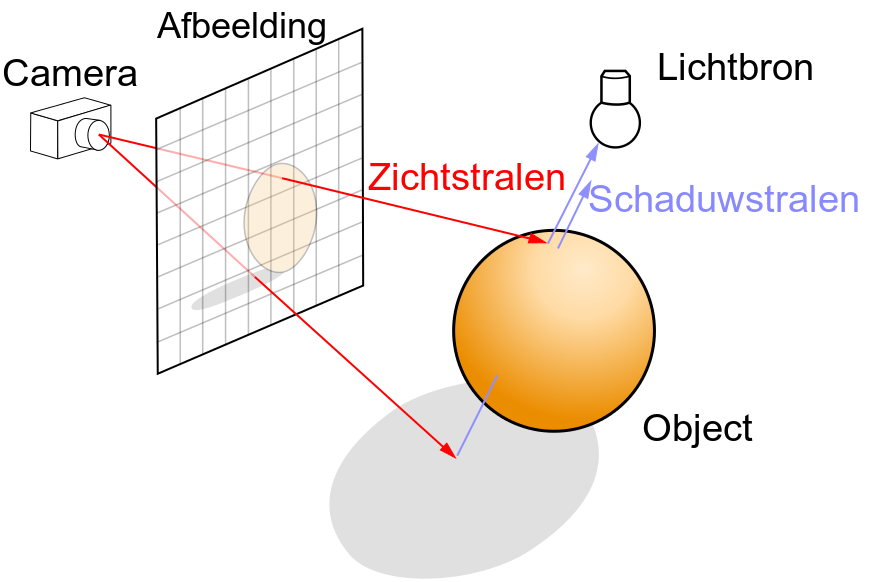
\includegraphics[width=0.5\linewidth]{img/ray-tracing}
        \caption[Visuele voorstelling van \textit{ray tracing}]%
    {Visuele voorstelling van \textit{ray tracing} - \small Door elke pixel worden één of meerdere zichtstralen gestuurd. Schaduwstralen worden gebruikt om de belichting in de scene realistisch te maken. Deze afbeelding is een aangepaste versie van een afbeelding op \url{https://en.wikipedia.org/wiki/Ray_tracing_(graphics)}}
        \label{fig:raytracing}    
    \end{figure}

    Om realistische afbeeldingen te maken, wordt belichting in rekening gebracht. De eenvoudigste vorm van belichting is directe belichting, een punt is donker als er niet rechtstreeks licht van een lichtbron op valt. Om dit te ondersteunen in \textit{ray tracing} wordt gebruikt gemaakt van schaduwstralen, stralen van het punt naar de lichtbron.  Deze schaduwstralen worden geïntersecteerd met de scene, als een intersectiepunt tussen het punt en de lichtbron gevonden wordt, is de lichtbron niet zichtbaar.  Bij elke intersectie wordt aan de hand van schaduwstralen gekeken of het punt belicht wordt of niet, als het niet belicht wordt, is de kleur zwart. Voor indirecte belichting kan een andere techniek, \textit{path tracing}, gebruikt worden. \textit{Path tracing} reflecteert stralen in het intersectiepunt afhankelijk van het materiaal en als deze straal na een aantal botsingen een lichtbron raakt, krijgt het intersectiepunt een belichting van die lichtbron.    
    
  %  , kleur intersectiepunt is kleur pixel -> path tracing.
  %  voor realistische beeldgeneratie + referentie,


    \paragraph{Acceleratiestructuren}
    Het doel van acceleratiestructuren is om het aantal straal-driehoek intersecties te verminderen.
    De simpelste acceleratiestructuur bestaat uit het omhullende volume van de scene.
    Testen op intersectie met de driehoeken in de scene gebeurt dan enkel als dit omhullende volume intersecteert met de straal.
    Deze acceleratiestructuur kan worden uitgebreid tot een boomstructuur door dit volume recursief op te delen in kindvolumes.
    Binaire bomen delen elk omhullend volume op in twee nieuwe volumes, andere acceleratiestructuren zoals bijvoorbeeld octrees, delen het volume op in meer dan twee volumes.
    \\

    Het volume kan worden opgedeeld op twee manieren: volgens objecten of volgens ruimte.
    Bij opdeling volgens objecten worden de objecten binnen het volume opgedeeld in meerdere disjuncte groepen en de kindvolumes zijn de omhullende volumes van deze groepen.
    Na deze opdeling zit elk object in exact één van deze nieuwe volumes, maar de volumes kunnen overlappen.
    Een voorbeeld van een acceleratiestructuur waarbij de opdeling volgens objecten gebeurt is de \textit{Bounding Volume Hierarchy} ($\symBVH$).
    Opdeling volgens ruimte betekent dat de ruimte in het volume wordt opgedeeld in meerdere delen.
    Na deze opdeling overlappen deze nieuwe volumes niet, maar een object ligt nu in minstens één (en mogelijks in meerdere) kindvolume(s).
    De $\symBSP$ boom deelt de ruimte van het volume steeds op in twee kindvolumes.
    % TODO: combinatie van Kd en BVH ? SBVH
    % TODO: check if all abbrev are listed and defined at first usage

\section{$\symBSP$ bomen}
    De $\symBSP$ boom deelt de ruimte van het omhullende volume recursief op door te splitsen volgens een willekeurig georiënteerd vlak totdat een bepaalde stopconditie bereikt is.
    Het feit dat de $\symBSP$ boom volgens willekeurig georiënteerde vlakken splitst, is zowel een voor- als nadeel.
    Het zorgt ervoor dat de $\symBSP$ boom zich heel goed kan aanpassen aan de scene en alle niet-intersecterende driehoeken in principe kan scheiden (zie figuur \ref{fig:splitsing-bsp}).
    Maar het zorgt er ook voor dat het heel moeilijk is om deze goede splitsingsvlakken te vinden.
    In de praktijk wordt vaak een specifieke soort $\symBSP$ boom gebruikt: de $\symKd$ boom.
    \begin{figure}
        \centering
        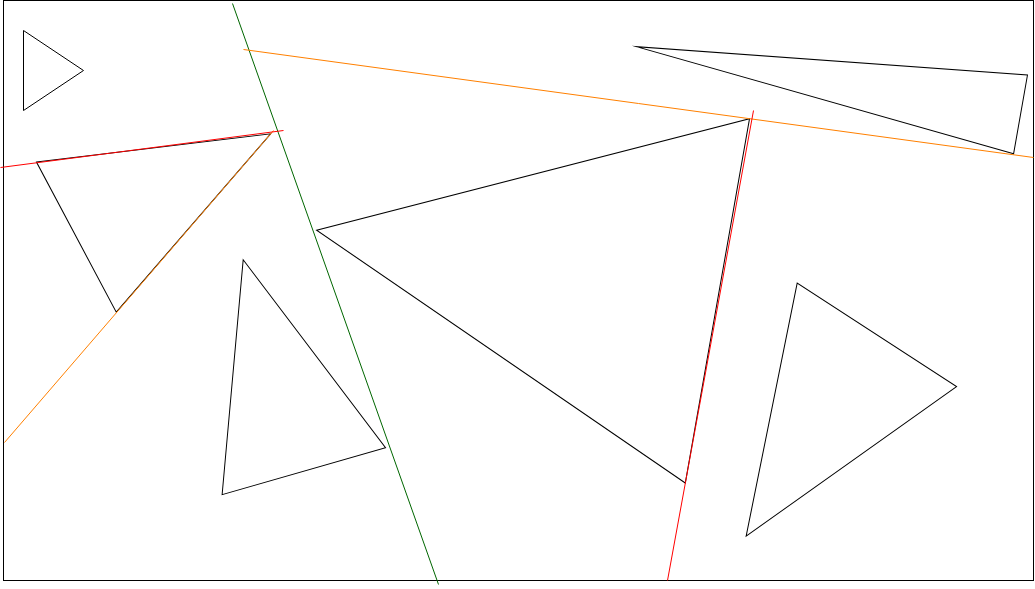
\includegraphics[width=\linewidth]{img/splitsing-BSP}
        \caption[Splitsingskracht $\symBSP$ boom]%
        {Splitsingskracht $\symBSP$ boom - \small Een 2D voorbeeld dat toont dat alle (niet-intersecterende) driehoeken gesplitst kunnen worden door een $\symBSP$ boom.}
        \label{fig:splitsing-bsp}    
    \end{figure}    
    \paragraph{Het bouwen van de boom}
    Het splitsingsvlak dat een knoop opdeelt in twee delen, kan een grote impact hebben op het aantal doorkruisstappen en het aantal driehoekintersecties.
    Het bouwalgoritme moet voor elke knoop het beste splitsingvlak bepalen en als splitsen volgens dat vlak voordelig is, de knoop opsplitsen in twee kindknopen.
    Heuristieken voorspellen hoe goed een splitsing volgens een bepaald splitsingsvlak is.   
    Het algoritme stopt met het splitsen van de knoop als een stopconditie bereikt wordt.
    Deze stopconditie kan een maximale diepte zijn, of het feit dat er geen nuttig splitsingsvlak gevonden wordt of dat het aantal driehoeken in de knoop lager is dan een vastgelegde limiet, bijvoorbeeld als er maar één driehoek in de knoop zit.

    %Spatiaal, opsplitsen volgens willekeurige vlakken
    %Niet feasible geacht
   
\section{$\symKd$ Bomen}   
    De $\symKd$ boom is een $\symBSP$ boom waarbij alle splitsingsvlakken asgealigneerd zijn.
    Hiermee wordt bedoeld dat de splitsingsrichting (de normaal op het splitsingsvlak) evenwijdig is aan één van de drie hoofdassen.
    Dit zorgt ervoor dat elke knoop van de boom een asgealigneerde balk voorstelt.
    Het doorkruisen van een knoop uit een $\symKd$ boom is daardoor goedkoper dan het doorkruisen van een knoop uit een algemene $\symBSP$ boom.
    De reden hiervoor is dat het goedkoper is om het intersectiepunt van een straal en een asgealigneerd vlak te vinden (verschil en vermenigvuldiging) dan het intersectiepunt van een straal en een willekeurig vlak (twee scalaire producten en deling).
    Door de beperking op mogelijke splitsingsvlakken kunnen $\symKd$ bomen zich minder goed aanpassen aan de scene.
    Ze kunnen bijvoorbeeld niet alle niet-intersecterende driehoeken scheiden. 
    Figuur \ref{fig:splitsing-kd} toont een situatie waarin de $\symKd$ boom niet alle driehoeken kan scheiden.
    \\

    \begin{figure}
        \centering
        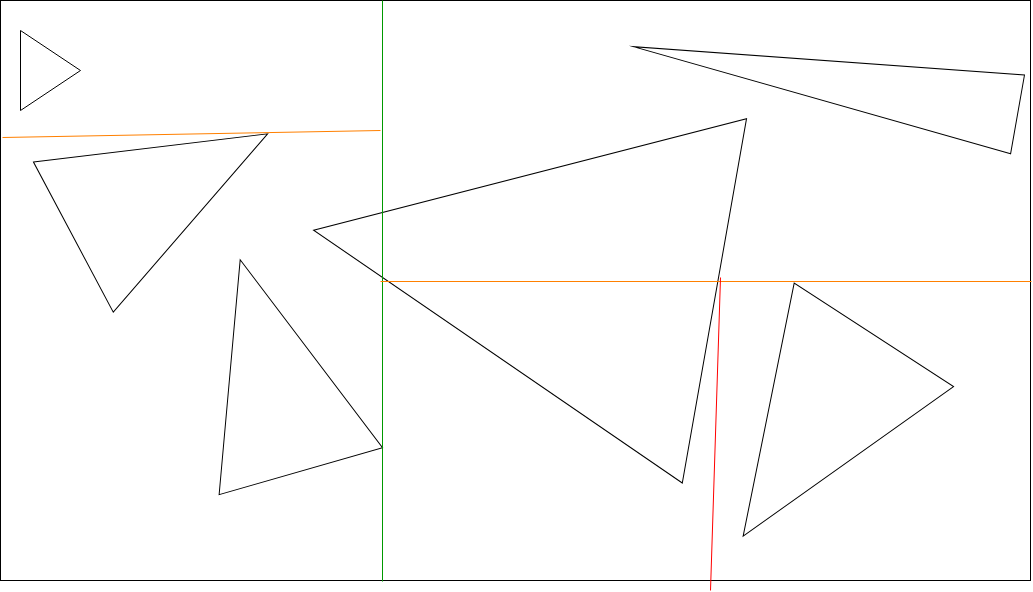
\includegraphics[width=\linewidth]{img/splitsing-Kd}
        \caption[Splitsingskracht $\symKd$ boom]{Splitsingskracht $\symKd$ boom - \small Een 2D voorbeeld dat toont dat niet alle (niet-intersecterende) driehoeken gesplitst kunnen worden door de asgealigneerde vlakken van de $\symKd$ boom. De twee driehoeken linksonder (en rechtsboven) kunnen niet gesplitst worden omdat zowel hun projecties op de x-as, als hun projecties op de y-as overlappen.}
        \label{fig:splitsing-kd}    
    \end{figure}

    Ondanks dit nadeel, worden in de praktijk $\symKd$ bomen verkozen boven algemene $\symBSP$ bomen.
    \authorIze{} \cite{ize} geven drie (volgens hun foute) ruimverspreide aannames over algemene $\symBSP$ bomen die ervoor zorgen dat $\symKd$ bomen hoger ingeschat worden.
    Ten eerste wordt er aangenomen dat algemene $\symBSP$ bomen nooit sneller kunnen zijn dan $\symKd$ bomen omdat het doorkruisen van een $\symBSP$ boom beduidend duurder is.
    De beperkte precisie van vlottende komma getallen wordt gezien als het tweede probleem omdat het $\symBSP$ bomen numeriek onstabiel zou maken.
    De derde aanname is dat door de grotere flexibileit (= grotere verzameling van mogelijke splitsingsvlakken) het veel moeilijker is om een $\symBSP$ boom te bouwen dan om een $\symKd$ boom te bouwen.
    \\

    Voor een Kd-boom is de Surface Area Heuristiek ($\symSAH$) de beste gekende methode om bomen met minimale verwachtte kost te bouwen.
    De $\symSAH$ is oorspronkelijk ontwikkelt door \authorGoldsmithSalmon{} \cite{goldsmith1987automatic} voor de $\symBVH$ en later aangepast door \authorMacDonaldBooth{} \cite{macdonald1990heuristics} voor de $\symKd$ boom. 
    De $\symSAH$ schat de kost van een splitsingsvlak door te veronderstellen dat beide kindknopen, bladknopen worden en dat de kost om een bladknoop te intersecteren afhankelijk is van het aantal driehoeken en de oppervlakte van het omhullende volume.
    De verwachte kost $\symCost$ om een knoop $\symNodeExample$ te splitsen in kindknopen ${\symLeft}$ en ${\symRight}$ is dan: $\symCost_\symNodeExample = \frac{\symSA(\symLeft)}{\symSA(\symNodeExample)}*\symNbPrimitives_\symLeft*\symCost_\symIntersection + \frac{\symSA(\symRight)}{\symSA(\symNodeExample)}*\symNbPrimitives_\symRight*\symCost_\symIntersection + \symCost_\symTraversal$ met kost $\symCost$, oppervlakte $\symSA()$ en aantal driehoeken $\symNbPrimitives$.
    De subscripts ${\symIntersection}$ en ${\symTraversal}$ staan voor respectievelijk intersectie en doorkruising.
    De kost van het beste splitsingsvlak (laagste kost) wordt dan vergeleken met de kost voor de knoop als die niet gesplitst zou worden: $\symNbPrimitives*\symCost_\symIntersection$.
    Als splitsen voordelig is, wordt de knoop opgesplitst volgens dit splitsingsvlak, anders wordt de knoop een bladknoop.
    \\

    Alle mogelijke asgealigneerde splitsingsvlakken testen is ondoenbaar. 
    \authorHavran{} \cite{havran2000heuristic} toonde aan dat de kost van de $\symSAH$ langs een richting ofwel lineair stijgt ofwel linear daalt tussen eindpunten (de minimale en maximale waarde) van de driehoeken langs die richting.
    Dit impliceert dat het beste splitsingsvlak door een eindpunt van een driehoek gaat.
    Het is dus voldoende om enkel de splitsingsvlakken te bekijken die door de eindpunten van de driehoeken gaan.
    Hieruit volgt dat er voor elke richting in een knoop met $n$ driehoeken, $2n$ splitsingsvlakken bekeken moeten worden.
    Bij een $\symKd$ boom is het dus voldoende om $6n$ splitsingsvlakken te bekijken.
    Om de $\symSAH$ kost te berekenen voor een splitsingsvlak moet het aantal driehoeken dat (deels) aan de ene kant van het splitsingsvlak ligt ($\symNbPrimitives_\symLeft$) en het aantal driehoeken dat (deels) aan de andere kant ligt ($\symNbPrimitives_\symRight$) gekend zijn.
    Om deze aantallen efficiënt te kunnen berekenen, worden de eindpunten van de driehoeken in de knoop gesorteerd volgens hun projectie op de splitsingsrichting.
    Een veegbeweging (\textit{sweep}) over deze gesorteerde lijst kan dan in lineaire tijd de $SAH$ kost van alle splitsingsvlakken langs de splitsingsrichting berekenen.

    % nulbonus ?
\section{$\symRBSP$ bomen}
    De Restricted Binary Space Partitioning ($\symRBSP$) boom is een uitbreiding van de $\symKd$ boom die toelaat om knopen op te splitsen volgens splitsingsrichtingen uit een vaste verzameling van k richtingen.
    Het omhullend volume van een $\symRBSP$ knoop is hierdoor geen balk maar een Discreet Geöriënteerde Polytoop met k richtingen: een \symKDOP.
    Zowel \authorKlosowki{} \cite{klosowski1998efficient} als \authorZachmann{} \cite{zachmann1998rapid} hebben hiërarchiën van \symKDOP s gebruikt binnen het domein van botsherkenning (\textit{collision detection}).
    De $\symRBSP$ boom is voor het eerst gebruikt in ray tracing door \authorKammaje{} \cite{Kammaje} en verder onderzocht door \authorBudge{} \cite{Budge}.
    Aangezien de splitsingsrichtingen niet asgealigneerd moeten zijn, lijkt de $\symRBSP$ boom meer op de algemene $\symBSP$ boom dan de $\symKd$ boom. Net als de $\symKd$ boom kan de $\symRBSP$ boom niet alle niet-intersecterende driehoeken scheiden. 
    Figuur \ref{fig:splitsing-rbsp} toont een situatie waarin de $\symRBSP$ boom niet alle driehoeken kan scheiden.
    \\

    \begin{figure}
        \centering
        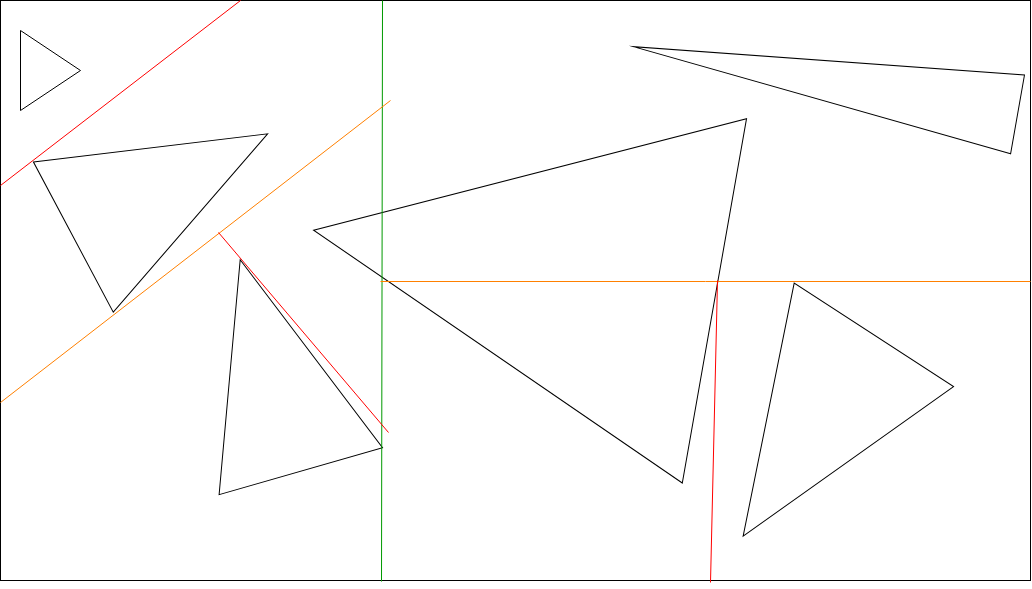
\includegraphics[width=\linewidth]{img/splitsing-RBSP}
        \caption[Splitsingskracht $\symRBSP$ boom]{Splitsingskracht $\symRBSP$ boom - \small Een 2D voorbeeld dat toont dat niet alle (niet-intersecterende) driehoeken gesplitst kunnen worden door de vlakken van de $\symRBSP$ boom. De $\symRBSP$ boom kan de driehoeken wel beter splitsen dan de $\symKd$ boom in figuur \ref{fig:splitsing-kd}. De twee driehoeken rechtsboven kunnen niet gesplitst worden omdat de discrete verzameling van k richtingen, geen richting bevat waarlangs deze driehoeken gesplitst kunnen worden.}
        \label{fig:splitsing-rbsp}    
    \end{figure}

    Een belangrijke ontwerpbeslissing bij $\symRBSP$ bomen is het kiezen van de verzameling splitsingsrichtingen. 
    Volgens \authorBudge{} \cite{Budge} werkt in principe elke verzameling met minstens drie niet-evenwijdige richtingen, maar is het gewenst om richtingen te kiezen die samen de eenheidsbol goed bedekken.
    \authorKammaje{} \cite{Kammaje} genereren punten langs een spiraal op gelijk verdeelde breedtegraden volgens de gouden ratio.
    \authorBudge{} \cite{Budge} gebruiken de verzamelingen die ze de standaard richtingen van \authorKlosowki{} \cite{klosowski1998efficient} noemen.
    Deze richtingen gebruiken enkel waarden uit de verzameling $\{-1, 0, 1\}$ als x, y en z coördinaat. %TODO meer uitwijden ?
    \\

    \authorKammaje{} \cite{Kammaje} toonden aan dat de SAH ook gebruikt kan worden voor $\symRBSP$ bomen. Net zoals bij de $\symKd$ boom moeten voor elke splitsingsrichting de eindpunten van de driehoeken gesorteerd worden en $2n$ splitsingsvlakken bekeken worden. In totaal bekijkt de $\symRBSP$ boom dus $2kn$ splitsingsvlakken. Het bouwen van de $\symRBSP$ boom is computationeel duurder dan het bouwen van de $\symKd$ boom door het grotere aantal richtingen en het feit dat het berekenen van de oppervlakte van een \symKDOP{} computationeel duurder is dan het berekenen van de oppervlakte van een balk. \authorBudge{} \cite{Budge} vonden een oplossing voor dit tweede probleem door een methode te ontwikkelen waarmee de oppervlaktes van de kind \symKDOP s incrementeel berekend kunnen worden tijdens het sweepen.\\

    De huidige $\symRBSP$ implementaties zijn superieur ten opzichte van de $\symKd$ boom in termen van het aantal driehoekintersecties en het aantal doorkruisingen, maar moet onderdoen in termen van rendertijd.
    \authorIze{} \cite{ize} menen dat de $\symRBSP$ boom de slechtste eigenschappen van zowel de $\symKd$ boom als de algemene $\symBSP$ boom overneemt. 
    Net als de $\symKd$ boom kan het geen rekening houden met de lokale geometrie en zich dus niet aanpassen aan complexe geometrie.
    Net als bij de algemene $\symBSP$ boom moet de intersectie met een willekeurig georiënteerd vlak berekend worden om knopen te doorkruisen. \authorBudge{} \cite{Budge} tonen aan dat deze tweede eigenschap minder erg is bij de $\symRBSP$ boom dan bij de algemene $\symBSP$ boom omdat het mogelijk is om alle scalaire producten op voorhand (en dus maar één keer) te berekenen.

\section{Algemene $\symBSP$ Bomen in de praktijk}
    \authorIze{} \cite{ize} ontwikkelden de eerste algemene $\symBSP$ boom voor raytracing. In tegenstelling tot de $\symKd$ en $\symRBSP$ boom kan $\symBSPize$ wel splitsingsvlakken kiezen afhankelijk van de geometrie. De $\symBSPize$ boom gebruikt de splitsingsvlakken van de $\symKd$ boom en elke driehoek in de knoop bepaalt nog vier extra splitsingsvlakken. Deze vier vlakken zijn: het vlak van de driehoek zelf (autoparitie) en de drie vlakken loodrecht op de driehoek door elk van de drie zijden. Merk op dat deze laatste vier vlakken rekening houden met de geometrie en niet mogelijk zouden zijn bij een $\symRBSP$ boom. Het omhullend volume van de knopen bij een $\symBSP$ boom is een convex veelvlak.
    Voor de eenvoud wordt de omhullende balk gebruikt als omhullend volume voor de wortelknoop. Dit heeft als extra voordeel dat er een zeer snelle test is voor stralen die niets raken. \\

    % sweeping Kd richtingen & bvh hulpstructuur
    De \symSAH{} kan ook gebruikt worden voor algemene $\symBSP$ bomen. De $\symBSPize$ boom controleert de $6n$ $\symKd$ splitsingsvlakken door te sweepen zoals bij de $\symKd$ en $\symRBSP$ boom. De $SA$ berekening is duurder aangezien het omhullende volume een convex veelvlak is. 
    De $\symBSPize$ boom controleert ook vier extra vlakken per driehoek. 
    Voor deze vlakken is het berekenen van de $SAH$ kost moeilijker omdat het aantal driehoeken links en rechts van het vlak bepaald moet worden. 
    Om dit efficiënt te bepalen gebruiken \authorIze{} \cite{ize} de $\symBVH$ als hulpstructuur. 
    In elke knoop wordt een $\symBVH$ boom gebouwd en die wordt bij elke niet-$\symKd$ splitsing gebruikt om het aantal driehoeken in beide kindknopen te bepalen.
    Hierdoor is het bouwen van de $\symBSPize$ boom computationeel beduidend duurder dan het bouwen van $\symRBSP$ en $\symKd$ bomen. 
    De inwendige knopen van de boom kunnen worden opgedeeld in twee groepen: de knopen die gesplitst worden door een $\symKd$ vlak en de knopen die gesplitst worden door een geometrie-afhankelijk $\symBSP$ vlak.
    Met $\symKd$ knopen worden de knopen uit de eerste groep bedoeld, met $\symBSP$ knopen die uit de tweede groep.\\

    \authorIze{} \cite{ize} verminderen het probleem van de tragere $\symBSP$ boom doorkruising door $\symKd$ knopen apart te behandelen bij het doorkruisen. 
    Als een $\symKd$ knoop doorkruist wordt, kan de intersectie met het splitsingsvlak berekend worden als de intersectie van de straal met een asgealigneerd vlak. 
    De boom die deze optimalisatie toepast, wordt aangeduid met $\symBSPizefastkd$.
    Het feit dat $\symKd$ knopen goedkoper zijn om te doorkruisen dan $\symBSP$ knopen, zorgt ervoor dat er voor deze twee soorten knopen een aparte doorkruiskost gebruikt moet worden in de $SAH$: $\symCostTraversalBSP$ en $\symCostTraversalKd$.
    Deze kosten rechtstreeks in de $SAH$ gebruiken, zorgt ervoor dat voornamelijk $\symBSP$ knopen gecreëerd worden.
    De reden hiervoor is dat de intersectieterm van de $SAH$ lineair varieert in het aantal driehoeken en die intersectieterm domineert snel de constante doorkruisterm waardoor $\symBSP$ splitsingen, die de driehoeken beter splitsen, gekozen worden.
    Deze lineaire afhankelijkheid is geen probleem als de $SAH$ enkel moet beslissen of een knoop gesplitst wordt of niet, maar wel als het moet bepalen of een knoop al of niet gesplitst wordt en of dit best door een goedkoep $\symKd$ vlak of door een duur $\symBSP$ vlak gedaan wordt.
    \authorIze{} \cite{ize} lossen dit probleem op door ook $\symCostTraversalBSP$ lineair te laten variëren in het aantal driehoeken: $\symCostTraversalBSP = \alpha * \symCost_\symIntersection * (\symNbPrimitives - 1) + \symCostTraversalKd$ waarbij $\alpha$ een instelbare parameter is.
    Als er na het testen van alle splitsingsvlakken geen splitsingsvlak gevonden is dat zorgt dat de kost om te splitsen lager is dan de kost om een bladknoop te creëren, worden alle $\symBSP$ vlakken opnieuw getest, maar deze keer met een constante $\symCostTraversalBSP$. Dit blijkt veel beter te werken dan een constante kost. Merk op dat deze optimalisatie gebruikt kan worden bij elke $\symBSP$ boom die de $\symKd$ richtingen bekijkt. Aangezien de $\symKd$ richtingen bij alle huidige $\symRBSP$ implementaties steeds in de verzameling splitsingsrichtingen zitten, kan de optimalisatie ook gebruikt worden om een $\symRBSPKd$ boom te bouwen.\\
    
    De $\symBSPizefastkd$ boom is in veel scenes even snel of zelfs sneller dan de $\symKd$ boom.
    De niet geöptimaliseerde $\symBSPize$ boom is voor sommige scenes ook al beter dan de $\symKd$ boom. 
    De winst wordt behaald door het lagere aantal straal driehoek intersecties.
    Het aantal knoop doorkruising stijgt echter, waardoor de totale verbetering wordt afgezwakt. De $\symBSPizefastkd$ boom toont veel minder variatie in rendertijd per pixel dan de $\symKd$ boom die duidelijke hotspot regio's heeft. Dit toont aan dat de $\symBSP$ boom beter kan omgaan met complexe geometrie.
    % amdahl ?

    %Voordelen
    %    Knopen kunnen beter worden opgesplist
    %Nadelen
    %    Duurder om te traversen
    %    Duurder om te bouwen (berekening SA van veelvlak vs SA van balk)
    %    Grote zoekruimte om beste splitsingsvlak te vinden
 
\section{Vergelijking}
\paragraph{Bouwen en intersecteren} 
Tabel \ref{tab:boom-vergelijking} vergelijkt de hierboven besproken $\symBSP$ bomen.
Hoe algemener de $\symBSP$ boom, hoe complexer het omhullend volume en hoe nauwer de boom kan aansluiten aan de scene.
Als voor elke driehoek in de knoop, dezelfde vlakken bekeken worden, kan sweeping toegepast worden om efficiënt de $SAH$ kosten te berekenen.
Als sweeping niet kan, zoals bij de geometrie-afhankelijke vlakken bij de $\symBSPize$ boom, is het berekenen van de $SAH$ kosten moeilijker en moet een hulpstructuur gebruikt worden.
Voor elk van deze soorten $\symBSP$ boom kan de optimalisatie met de snelle $\symKd$ knoop doorkruising gebruikt worden. Voor de $\symRBSP$ boom is dit nog nooit gedaan.

\begin{table}[tb]
    \centering
    \begin{tabular}{@{}|l|c|c|c|@{}} \toprule      
            & $\symKd$     & $\symRBSP$ & $\symBSPize$ \\ \midrule
      Omhullend volume & Asgealigneerde balk & $\symKDOP$ & Convex veelvlak \\
      Sweeping                              &  Ja   & Ja & Deels    \\
      Geometrie afhankelijke vlakken & Nee & Nee & Ja \\
      Snelle Kd doorkruising                 & $\symKd$  & $\symRBSPKd$ \footnotemark[1] & $\symBSPizefastkd$    \\
      \# splitsingsvlakken per niveau       &  $6n$   & $2kn$ & $10n$  \\
      totaal \# $\neq$ splitsingsvlakken           &  $6n$   & $2kn$ & $10n$     \\ \bottomrule
    \end{tabular}
    \caption{Vergelijking van de bestaande soorten $\symBSP$ bomen. }
    \label{tab:boom-vergelijking}
  \end{table}
  \footnotetext[1]{De $\symRBSPKd$ boom is nog nooit geïmplementeerd.}


  \paragraph{Aantal verschillende splitsingsvlakken}
  Eén van de belangrijkste eigenschappen van een $\symBSP$ algoritme is zijn vermogen om zich aan te passen aan complexe geometrie.
  Het totaal aantal verschillende splitsingsvlakken dat bekeken wordt tijdens het bouwen van de boom, draagt bij tot dit vermogen.
  Voor een scene met $n$ driehoeken, bekijkt een $\symKd$ boom $6n$ verschillende splitsingsvlakken. 
  Elk niveau van de boom bekijkt exact dezelfde splitsingsvlakken. Figuur \ref{fig:splitsingsvlakken-kd} toont dit visueel.
  Een $\symRBSP$ boom met k discrete richtingen doet hetzelfde, maar bekijkt $2kn$ verschillende splitsingsvlakken. 
  Figuur \ref{fig:splitsingsvlakken-rbsp} toont dit visueel.
  De $\symBSPize$ boom gebruikt $10n$ verschillende splitsingsrichtingen, $6n$ voor de $\symKd$ richtingen en $n$ voor elk van de vier andere richtingen.
  De $\symBSPize$ boom bekijkt op elk niveau ook exact dezelfde splitsingvlakken en is dus niet zo algemeen als een $\symBSP$ boom kan zijn. 
  Figuur \ref{fig:splitsingsvlakken-bspize} toont dit visueel.
  De reden hiervoor is dat de gebruikte $\symBSP$ splitsingsvlakken enkel afhankelijk zijn van de driehoeken zelf en niet van welke driehoeken samen in een knoop zitten.
  Geen van bovenstaande bomen gebruikt de volledige vrijheid van een $\symBSP$ boom om op elk niveau andere splitsingsvlakken te nemen en op die manier beperken ze hun vermogen om zich aan te passen aan complexe geometrie.
  Driehoeken die in de wortelknoop door geen enkel vlak van elkaar kunnen worden gesplitst, kunnen nooit van elkaar gesplitst worden.
  Het volgende hoofdstuk introduceert nieuwe $\symBSP$ bomen die deze vrijheid wel benutten.
  
  \tikzset{every tree node/.style={minimum width=2em,draw,circle},
  blank/.style={draw=none},
  edge from parent/.style=
  {draw,edge from parent path={(\tikzparentnode) -- (\tikzchildnode)}},
  level distance=1.5cm}
  \begin{figure}
    \centering
    \begin{subfigure}[t]{.3\linewidth}
        
  \resizebox{\textwidth}{!}{%
\begin{tikzpicture}
\Tree
[ .\node[shading = axis, left color=nodeblue1, right color=nodered2,shading angle=90, text=white]{$6n$};    
[.\node[shading = axis, left color=nodeblue1, right color=nodeblue2,shading angle=90, text=white]{$6\frac{n}{2}$};
 [.\node(n3l)[fill=nodeblue1]{$6\frac{n}{4}$};]
 [.\node[fill=nodeblue2, text=white]{$6\frac{n}{4}$};]
]
[.\node[shading = axis, left color=nodered1, right color=nodered2,shading angle=90, text=white]{$6\frac{n}{2}$};
 [.\node[fill=nodered1, text=white]{$6\frac{n}{4}$};]
 [.\node(n3r)[fill=nodered2, text=white]{$6\frac{n}{4}$};]
]
]
\node at (3,0.5) {$\#$};
\node at (4,0.5) {$\# \neq$};
\node at (3,0) {$6n$};
\node at (3,-1.5) {$6n$};
\node at (3,-3) {$6n$};
\node at (4,0) {$6n$};
\node at (4,-1.5) {$6n$};
\node at (4,-3) {$6n$};
\end{tikzpicture}
}
\caption{$\symKd$ boom}
\label{fig:splitsingsvlakken-kd}
\end{subfigure}
\begin{subfigure}[t]{.3\linewidth}
\resizebox{\textwidth}{!}{%
\begin{tikzpicture}
\Tree
[ .\node[shading = axis, left color=nodeblue1, right color=nodered2,shading angle=90, text=white]{$2kn$};    
[.\node[shading = axis, left color=nodeblue1, right color=nodeblue2,shading angle=90, text=white]{$2k\frac{n}{2}$};
 [.\node(n3l)[fill=nodeblue1]{$2k\frac{n}{4}$};]
 [.\node[fill=nodeblue2, text=white]{$2k\frac{n}{4}$};]
]
[.\node[shading = axis, left color=nodered1, right color=nodered2,shading angle=90, text=white]{$2k\frac{n}{2}$};
 [.\node[fill=nodered1, text=white]{$2k\frac{n}{4}$};]
 [.\node(n3r)[fill=nodered2, text=white]{$2k\frac{n}{4}$};]
]
]
\node at (3,0.5) {$\#$};
\node at (4,0.5) {$\# \neq$};
\node at (3,0) {$2kn$};
\node at (3,-1.5) {$2kn$};
\node at (3,-3) {$2kn$};
\node at (4,0) {$2kn$};
\node at (4,-1.5) {$2kn$};
\node at (4,-3) {$2kn$};
\end{tikzpicture}
}
\caption{$\symRBSP$ boom}
\label{fig:splitsingsvlakken-rbsp}
\end{subfigure}
\begin{subfigure}[t]{.3\linewidth}
\resizebox{\textwidth}{!}{%
\begin{tikzpicture}
\Tree
[ .\node[shading = axis, left color=nodeblue1, right color=nodered2,shading angle=90, text=white]{$10n$};    
[.\node[shading = axis, left color=nodeblue1, right color=nodeblue2,shading angle=90, text=white]{$10\frac{n}{2}$};
 [.\node(n3l)[fill=nodeblue1]{$10\frac{n}{4}$};]
 [.\node[fill=nodeblue2, text=white]{$10\frac{n}{4}$};]
]
[.\node[shading = axis, left color=nodered1, right color=nodered2,shading angle=90, text=white]{$10\frac{n}{2}$};
 [.\node[fill=nodered1, text=white]{$10\frac{n}{4}$};]
 [.\node(n3r)[fill=nodered2, text=white]{$10\frac{n}{4}$};]
]
]
\node at (3,0.5) {$\#$};
\node at (4,0.5) {$\# \neq$};
\node at (3,0) {$10n$};
\node at (3,-1.5) {$10n$};
\node at (3,-3) {$10n$};
\node at (4,0) {$10n$};
\node at (4,-1.5) {$10n$};
\node at (4,-3) {$10n$};
\end{tikzpicture}
}
\caption{$\symBSPize$ boom}
\label{fig:splitsingsvlakken-bspize}
\end{subfigure}
\caption[Splitsingsvlakken $\symKd$, $\symRBSP$ en $\symBSPize$]{Splitsingsvlakken $\symKd$, $\symRBSP$ en $\symBSPize$ - \small Per niveau het aantal ($\#$) splitsingsvlakken en het totaal aantal verschillende ($\# \neq$) splitsingsvlakken gebruikt in bovenliggende niveaus.}
%TODO: meer uitleg
\end{figure}

%%% Local Variables: 
%%% mode: latex
%%% TeX-master: "masterproef"
%%% End: 
